% create the chapter theoretical background
\chapter{Theoretical Background}

% section about antibiotic resistance
\section{Antibiotic resistance}

Antibiotic resistance is definied as the the ability of bacteria, viruses, fungi and parasites resists the antimicrobial medicines like for example antibiotics \cite{who_antibiotic_resistance}. Most commonly used antibiotics are the so called $\beta$-lactam antibiotics which contain a $\beta$-lactam ring in their chemical structure \cite{bush2013}. The $\beta$-lactam ring is a four membered ring ring with a carbonyl group. This includes penicillin, cephalosporin, carbapenems, which are the most common antibiotics used today \cite{versporten2018}. The core structure of penicillin derivates \textbf{1} and cephalosporin derivates \textbf{2} are shown in Figure \ref{fig:beta_lactam_antibiotics}.

\begin{figure}[htbp]
    \centering
    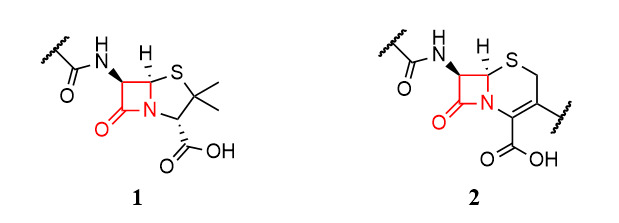
\includegraphics[width=0.6\textwidth]{resources/images/beta_lactam_antibiotics_example.jpeg}
    \caption{Core structure of $\beta$-lactam antibiotics. The four-membered $\beta$-lactam ring is the key structural element responsible for the antibiotic activity (marked in red).}
    \label{fig:beta_lactam_antibiotics}
\end{figure}

The $\beta$-lactam antibiotics exert their bactericidal effect by targeting the bacterial cell wall. They mimic the the D-Ala-D-Ala moiety of the peptidoglycan layer of the cell wall, which is the main component of the cell wall in bacteria. The peptidoglycan layer is build from carbohydrates of repeating units N-acetylglucosamine (GlcNAc) and N-acetylmuramic acid (MurNAc), which are linked by a diverse component. The active site performs a nucleophilic attack on the D-Ala of the pentapetide linked to the MurNAc. The weakend cell is not longer able to withstand the osmotic pressure, leading to the cell lysis and death \cite{kim2023}.

Due to evolutionary pressure, bacteria can develop resistance against the $\beta$-lactam antibiotics. The enzymes in both Gram-positive and Gram-negative bacteria which are responsible for the resistance are called $\beta$-lactamases. Through hydrolysis, the enzymes break the $\beta$-lactam ring, which is the key structure of the $\beta$-lactam antibiotics \cite{ambler1980}.
Based on the catalytic mechanism, the $\beta$-lactamases are classified into serine $\beta$-lactamases and metallo-$\beta$-lactamases. The former employ a active site with a serine residue, while the latter have a metal ion in their active site (typically zinc) \cite{kim2023} \cite{ambler1980}. Based on a proposed classification by sequence homology \cite{bush2013} the $\beta$-lactamases are classified into 4 classes, A, B, C and D. The classes A, C, and D include the serine $\beta$-lactamases, while the class B contains the metallo-$\beta$-lactamases \cite{bush2013}.


% section about machine learning
\section{Machine learning}

